% LaTeX file for resume
\documentclass[11pt, a4paper, french]{article}
\usepackage[francais]{babel}
\usepackage[utf8]{inputenc}


\usepackage[usenames, dvipsnames]{xcolor}

\usepackage[framemethod=tikz]{mdframed}
\newmdenv[innerlinewidth=0.8pt, roundcorner=4pt,linecolor=RoyalBlue,innerleftmargin=6pt,
innerrightmargin=6pt,innertopmargin=6pt,innerbottommargin=6pt]{mybox}
\usepackage{wrapfig}


\usepackage{etaremune}


\usepackage[colorlinks = true,urlcolor = BrickRed]{hyperref}

\usepackage{eurosym}


\usepackage{datetime}
\newdateformat{yeardate}{\THEYEAR}

\usepackage{fancyhdr}  % use this package to get a 2 line header
\renewcommand{\headrulewidth}{0pt} % suppress line drawn by default by fancyhdr

\pagestyle{fancy}     % set pagestyle for document
\usepackage{lastpage}
% \cfoot{ \thepage}
% \setcounter{page}{3}
\rhead{\textcolor{gray}{ \thepage/\pageref*{LastPage}}}
\cfoot{}
\rfoot{\href{https://johanmazoyer.github.io/}{johanmazoyer.github.io}}
\rhead{}


\setlength{\headwidth}{17.2cm} % taille de l'entete
\usepackage[total={17.2cm,25.cm}, left=1.9cm, top=2.5cm]{geometry}
\setlength{\parindent}{0pt} 


\begin{document}
\lfoot{\textcolor{Gray}{CV mis à jour en \yeardate\today}}

\begin{huge}
\noindent\textbf{Johan MAZOYER}
\end{huge}\\

\textbf{Intérêts de recherche:} Instrumentation Optique, Imagerie Directe et Coronographie,
Observation et Caractérisation de Systèmes Extrasolaires, Disques de Débris\\



%%%%%%%%%%%%%%%%%%%%%%%%%%%%%%%%%%%%%%%%%%%%%%%%%%%%%%%%%%%%%%%%%%%%%%%%%%%%%%%%%%%%%%%%%%%%%%%%%%%%%%%%%%%%%%%%%%%%%%%%
%%%%%% SECTION RESEARCH EXPERIENCE
%%%%%%%%%%%%%%%%%%%%%%%%%%%%%%%%%%%%%%%%%%%%%%%%%%%%%%%%%%%%%%%%%%%%%%%%%%%%%%%%%%%%%%%%%%%%%%%%%%%%%%%%%%%%%%%%%%%%%%%%


\vspace{-0.8cm}
\textcolor{RoyalBlue}{\section{\large EXPÉRIENCES PROFESSIONNELLES}
\vspace{-0.2cm}\hrule}
\vspace{0.4cm}


\textbf{Chargé de recherche CNRS} --
\href{http://www.obspm.fr}{\textbf{LESIA/Observatoire de Paris}} (France)
\hfill     	 { \bf Depuis 2020}\\

\vspace{-0.05cm}
\textbf{NASA Sagan Fellow} --
\href{https://www.jpl.nasa.gov/}{\textbf{NASA Jet Propulsion Laboratory}} (Pasadena, CA)
\hfill      { \bf 2018 - 2019}\\

\vspace{-0.05cm}
\textbf{Post-doctorant} --
\href{http://physics-astronomy.jhu.edu/}{\textbf{Johns Hopkins University}} (Baltimore, MD)
\hfill   	 { \bf 2016 - 2018}\\

\vspace{-0.05cm}
\textbf{Post-doctorant} --
\href{http://www.stsci.edu}{\textbf{Space Telescope Science Institute}} (Baltimore, MD)
\hfill        { \bf 2014 - 2016}\\\

\vspace{-0.05cm}
\textbf{Doctorant} --
\href{http://www.obspm.fr/}{\textbf{LESIA/Observatoire de Paris}} (France)
\hfill        { \bf 2011 - 2014}\\


% \textbf{Jet Propulsion Laboratory} (JPL)  \hfill       {\small Pasadena, CA, USA} \\
% {\small \textit{Carl Sagan Fellow}}  \hfill  	 {\small \bf 2018 -- Présent}\\

% \vspace{-0.2cm}
% \hspace{0.5cm} \parbox{0.9\linewidth}{
%    \begin{itemize} \itemsep -3pt % reduce space between items
%    \vspace{-0.4cm}
%     \item \small Astrophysique : Caractérisation de disques avec GPI et WFIRST
%    \item \small Instrumentation : Développement de techniques instrumentales sur banc optique
%  \end{itemize} }\\

% \textbf{Johns Hopkins University} (JHU) \hfill       {\small Baltimore, MD, USA} \\
% {\small \textit{Chercheur post-doctoral}; superviseur : Christine Chen}  \hfill  	 {\small \bf 2016 -- 2018}\\

% \vspace{-0.4cm}
% \hspace{0.5cm} \parbox{0.9\linewidth}{
%    \begin{itemize} \itemsep -3pt % reduce space between items
%    \vspace{-0.2cm}
%     \item \small Astrophysique : Large programme sur les disques de débris sur GPI
%    \item \small Instrumentation : Méthodes deux miroirs pour l'imagerie haut-contraste
%  \end{itemize} }\\

% \vspace{-0.2cm}
% \textbf{Space Telescope Science Institute} (STScI) \hfill       {\small Baltimore, MD, USA} \\
% {\small \textit{Chercheur post-doctoral}; superviseur : Laurent Pueyo}  \hfill  	 {\small \bf 2014 --2016}\\

% \vspace{-0.4cm}
% \hspace{0.5cm} \parbox{0.9\linewidth}{
%    \begin{itemize} \itemsep -3pt % reduce space between items
%    \vspace{-0.2cm}
%     \item \small Astrophysique : Imagerie directe de disques (NICMOS, NICI, SPHERE)
%    \item \small Instrumentation : Correction active d'ouvertures de télescopes complexes \\

%  \end{itemize} }

% \vspace{-0.2cm}
% \textbf{Laboratoire d'études spatiales et d'instrumentation en astrophysique} (LESIA)  \hfill        {\small Paris, FR} \\
% {\small \textit{Doctorant}; encadrants : Pierre Baudoz et Gérard Rousset}  \hfill  	 	 {\small \bf 2011 -- 2014}\\
% \vspace{-0.1cm}
% \hspace{0.5cm} \parbox{0.9\linewidth}{
% \vspace{0.2cm}
% \small  Développement d'un senseur de front d'onde haut-contraste et imagerie\\ de disques de débris (Gemini/NICI)} \\

% \vspace{0.2cm}
% \textbf{Los Alamos National Laboratory} (LANL) \hfill    	Los Alamos, NM, USA\\
% {\small \textit{Étudiant de M2}; encadrants : Roger C. Wiens et Jérémie Lasue
%  \hfill  		 {\bf 2011}}\\
%  \vspace{-0.4cm}
% \hspace{0.5cm} \parbox{0.9\linewidth}{
% \small  MSL/ChemCam : Influence de l'atmosphère martienne sur les limites de détection} \\

% \vspace{0.1cm}
% \textbf{Institut de Recherche en Astrophysique et Planétologie} (IRAP) \hfill    	Toulouse, FR\\
% {\small \textit{Étudiant de M2}; encadrants:  Sylvestre Maurice et Olivier Gasnault
%  \hfill  		 {\bf 2011}}\\
%  \vspace{-0.4cm}
% \hspace{0.5cm} \parbox{0.9\linewidth}{
% \small  MSL/ChemCam : Influence de l'atmosphère sur les mesures du LIBS} \\

%\vspace{0.1cm}
% \textbf{CNES} \hfill    	Toulouse, France\\
%{\small \textit{Étudiant de M1}; Satellites Pleiades : simulation de composants de vol\hfill  		 {\bf Mars -- Juil. 2010}}\\
%
%\vspace{-0.3cm}
%\textbf{Le Relais} (Emmaüs) \hfill    		  Koudougou, Burkina Faso\\
%{\small Stage humanitaire\hfill  		  {\bf Juil. -- Sept. 2009}}	\\

%%%%%%%%%%%%%%%%%%%%%%%%%%%%%%%%%%%%%%%%%%%%%%%%%%%%%%%%%%%%%%%%%%%%%%%%%%%%%%%%%%%%%%%%%%%%%%%%%%%%%%%%%%%%%%%%%%%%%%%%
%%%%%% SECTION EDUCATION
%%%%%%%%%%%%%%%%%%%%%%%%%%%%%%%%%%%%%%%%%%%%%%%%%%%%%%%%%%%%%%%%%%%%%%%%%%%%%%%%%%%%%%%%%%%%%%%%%%%%%%%%%%%%%%%%%%%%%%%%

\vspace{-0.3cm}
\textcolor{RoyalBlue}{\section{\large FORMATION}
\vspace{-0.2cm}\hrule}
\vspace{0.4cm}

{\bf Doctorat} -- \href{https://www.univ-paris-diderot.fr/}{\textbf{Universit\'e Paris Diderot}}
\hfill Paris, France\\
{\small \it Astronomie et Astrophysique} \hfill  {\small \bf Septembre 2014}\\
{\footnotesize
\it Sujet : Haut contraste pour l'imagerie directe d'exoplanètes et de disques (P. Baudoz \& G. Rousset)}\\


\vspace{-0.05cm}
{\bf Master 2} --
\href{http://ezomp2.omp.obs-mip.fr/asep/index.php/fre}{\textbf{Université Paul Sabatier} }
 \hfill Toulouse, France\\
{\small \it Astrophysique, Science de l'Espace, Planétologie} \hfill { \small \bf Septembre 2011}\\
{\footnotesize
\it Stage : Influence de l'atmosphère martienne sur les limites de détection de MSL/Chemcam (O. Gasnault)}\\

\vspace{-0.05cm}
{\bf Diplôme d'ingénieur} -- \href{https://www.isae-supaero.fr/}{\textbf{\textbf{ISAE Supaero} }}  \hfill Toulouse, France\\
{\small \it Systèmes Spatiaux et Techniques d'Imageries Spatiales} \hfill { \small \bf Septembre 2011}\\


\vspace{-0.05cm}
{\bf Diplôme d'ingénieur} --
\href{http://www.polytechnique.edu/}{\textbf{\textbf{Ecole polytechnique} }}
\hfill Palaiseau, France  \\
{\small \it Systèmes Embarqués (électronique et informatique)}   \hfill {\small \bf Septembre 2011}\\

%%%%%%%%%%%%%%%%%%%%%%%%%%%%%%%%%%%%%%%%%%%%%%%%%%%%%%%%%%%%%%%%%%%%%%%%%%%%%%%%%%%%%%%%%%%%%%%%%%%%%%%%%%%%%%%%%%%%%%%%
%%%%%% SECTION AWARDS
%%%%%%%%%%%%%%%%%%%%%%%%%%%%%%%%%%%%%%%%%%%%%%%%%%%%%%%%%%%%%%%%%%%%%%%%%%%%%%%%%%%%%%%%%%%%%%%%%%%%%%%%%%%%%%%%%%%%%%%%

\vspace{-0.3cm}
\textcolor{RoyalBlue}{\section{\large BOURSES \& PRIX}
\vspace{-0.2cm}\hrule}
\vspace{0.4cm}

\textbf{Programme de Collaboration Franco-Chilienne} \href{https://www.univ-paris13.fr/ecos-sud/}{EcosSud} avec {\it Universidad de Chile} -- 3 ans \hfill   \textbf{2020}\\ %- \$300K/3 yrs

\vspace{-0.15cm}
\textbf{NASA Group Award}: LBTI Hosts Survey Science Team \hfill   \textbf{2020}\\ 

\vspace{-0.15cm}
\textbf{Carl Sagan Fellowship} (\href{http://www.stsci.edu/stsci-research/fellowships/nasa-hubble-fellowship-program}{NASA Hubble Fellowship Program}) -- 3 ans \hfill   { \bf 2018}\\

\vspace{-0.15cm}
Couverture du journal \textbf{Astronomy \& Astrophysics} (\href{https://www.aanda.org/articles/aa/abs/2014/04/contents/contents.html}{Volume 564}) \hfill  { \bf 2014}\\

% \vspace{-0.15cm}
% \textbf{Meilleure présentation}, conférence des chercheurs du CNES (JC2) \hfill   { \bf 2013}\\

\vspace{-0.15cm}
\textbf{Bourse doctorale} du CNES -- 3 ans \hfill   { \bf 2011}\\

% \vspace{-0.15cm}
% \textbf{Bourse d'étude} de l'Ecole polytechnique -- 4 ans \hfill   { \bf 2007}\\

%%%%%%%%%%%%%%%%%%%%%%%%%%%%%%%%%%%%%%%%%%%%%%%%%%%%%%%%%%%%%%%%%%%%%%%%%%%%%%%%%%%%%%%%%%%%%%%%%%%%%%%%%%%%%%%%%%%%%%%%
%%%%%% SECTION VULGARISATION
%%%%%%%%%%%%%%%%%%%%%%%%%%%%%%%%%%%%%%%%%%%%%%%%%%%%%%%%%%%%%%%%%%%%%%%%%%%%%%%%%%%%%%%%%%%%%%%%%%%%%%%%%%%%%%%%%%%%%%%%

% \newpage
% \textcolor{white}{.}
\vspace{-0.3cm}
\textcolor{RoyalBlue}{\section{\large DIFFUSION DES SCIENCES}
\vspace{-0.2cm}\hrule}
\vspace{0.4cm}
\begin{wrapfigure}{r}{0.19\textwidth}
\vspace{-0.8cm}
\begin{mybox}
    
\includegraphics[width=1.\textwidth]{figures_CV/PodcastScience.png}
 \end{mybox}
\vspace{-0.8cm}
\end{wrapfigure}
\textbf{Podcast Science} \\
\vspace{-0cm}
\hspace{0.3cm}
J'anime chaque semaine \href{http://www.podcastscience.fm}{PodcastScience.fm},
\textbf{émission scientifique hebdomadaire de radio} (podcast) d'une heure et demie à
3h. Le podcast produit des émissions sur tous les domaines scientifiques et je réalise tous les contenus
relatifs à la physique et à l'astrophysique.

\vspace{0.4cm}
\textbf{Conférences grand public}   \\
\hspace{0.3cm} CERN (Genève) et Palais de la découverte (Paris)\\


%%%%%%%%%%%%%%%%%%%%%%%%%%%%%%%%%%%%%%%%%%%%%%%%%%%%%%%%%%%%%%%%%%%%%%%%%%%%%%%%%%%%%%%%%%%%%%%%%%%%%%%%%%%%%%%%%%%%%%%%
%%%%%% SECTION TEACHING EXPERIENCE
%%%%%%%%%%%%%%%%%%%%%%%%%%%%%%%%%%%%%%%%%%%%%%%%%%%%%%%%%%%%%%%%%%%%%%%%%%%%%%%%%%%%%%%%%%%%%%%%%%%%%%%%%%%%%%%%%%%%%%%%

\vspace{-0.8cm}
\textcolor{RoyalBlue}{\section{\large ENCADREMENTS}
\vspace{-0.2cm}\hrule}
\vspace{0.4cm}
\textbf{Vito Squicciarini} (Postdoc, LESIA): co-encadrement avec A.-M. Lagrange \hfill \textbf{Depuis 2022}\\
\textbf{Yann Gutierrez} (PhD, LESIA): co-encadrement avec L. Mugnier, ONERA \hfill \textbf{Depuis 2022}\\
\textbf{Iva Laginja} (Postdoc, LESIA): CNES post-doctoral Fellow \hfill \textbf{Depuis 2022}\\
\textbf{Sophia Stasevic} (PhD, LESIA) co-encadrement avec A.-M. Lagrange and J. Milli \hfill \textbf{Depuis 2021}\\
% \textbf{Justin Hom} (PhD, ASU) co-encadrement avec J. Patience \hfill \textbf{Depuis 2020}\\
% \textbf{Kevin Fogarty} (PhD, JHU) co-encadrement avec L. Pueyo \hfill \textbf{2017-2019}\\

% \newpage
\vspace{-0.1cm}
\textcolor{RoyalBlue}{\section{\large ENSEIGNEMENT}
\vspace{-0.2cm}\hrule}
\vspace{0.4cm}
% \vspace{-0.2cm}
Cours de Master (Observatoire de Paris):
\begin{itemize} \itemsep -2pt
    \item[$\bullet$] Instrumentation for Astronomy 
    \item[$\bullet$] Detection of Exoplanets (collab. Anne-Marie Lagrange)
\end{itemize}


%%%%%%%%%%%%%%%%%%%%%%%%%%%%%%%%%%%%%%%%%%%%%%%%%%%%%%%%%%%%%%%%%%%%%%%%%%%%%%%%%%%%%%%%%%%%%%%%%%%%%%%%%%%%%%%%%%%%%%%%
%%%%%% campagnes d’observations
%%%%%%%%%%%%%%%%%%%%%%%%%%%%%%%%%%%%%%%%%%%%%%%%%%%%%%%%%%%%%%%%%%%%%%%%%%%%%%%%%%%%%%%%%%%%%%%%%%%%%%%%%%%%%%%%%%%%%%%%

% \vspace{-0.4cm}
% \textcolor{RoyalBlue}{\section{\large CAMPAGNES D'OBSERVATIONS}
% \vspace{-0.3cm}\hrule}
% \vspace{0.3cm}

% \textbf{Palomar Observatory (200 inch telescope)}
% \begin{itemize} \itemsep -1pt % reduce space between items
% 	    \item \small Mai 2015, 3 nuits -- Premiers tests sur télescope de la Self-Coherent Camera
% \end{itemize}

% \textbf{Gemini South/GPI}
% 	\begin{itemize} \itemsep -1pt % reduce space between items
% 	    \item \small Décembre 2015 - Novembre 2018 --	25 nuits en cumulé pour le large programme disque ou le programme de temps garanti du consortium GPI. Depuis fin 2016, toutes les observations Gemini sud sont menées à distance. J'ai effectué la majorité de mes observations à distance depuis Berkeley, le JPL et le STScI.
% \end{itemize}



%%%%%%%%%%%%%%%%%%%%%%%%%%%%%%%%%%%%%%%%%%%%%%%%%%%%%%%%%%%%%%%%%%%%%%%%%%%%%%%%%%%%%%%%%%%%%%%%%%%%%%%%%%%%%%%%%%%%%%%%
%%%%%% Demandes de temps
%%%%%%%%%%%%%%%%%%%%%%%%%%%%%%%%%%%%%%%%%%%%%%%%%%%%%%%%%%%%%%%%%%%%%%%%%%%%%%%%%%%%%%%%%%%%%%%%%%%%%%%%%%%%%%%%%%%%%%%%

% \newpage
% \textcolor{white}{.}
% \vspace{-0.8cm}
% \textcolor{RoyalBlue}{\section{\large DEMANDES DE TEMPS D'OBSERVATION ACCEPTÉES}
% \vspace{-0.3cm}\hrule}
% \vspace{0.3cm}

% \textbf{GEMINI South/GPI} : Membre du consortium GPI depuis septembre 2016
% \vspace{0.3cm}
% \begin{itemize} \itemsep -1pt % reduce space between items
%     \item \small GS-2015B-LP-6 ``Characterizing Dusty Debris in Exoplanetary Systems'' (PI: C. Chen)
%     \item \small DT-2019A-009 ``Decoding the Asymmetric Scattered Light Around HD 15115'' (PI: C. Chen)
%     \item \small GS-2019A-Q-109 ``Completing a Survey for Resolved Debris Disks in the Sco-Cen Assoc.'' (PI: J. Patience)
% \end{itemize}


% \textbf{VLT/SPHERE}
% %\vspace{-0.2cm}
% \begin{itemize} \itemsep -1pt % reduce space between items
% 	\item \small P 0101.C-0128 ``Resolving multiple belts and sub-structures in inner regions of highly inclined debris disks" (PI : A. Boccaletti)
%     \item \small P 098.C-0686 ``Resolving sub-structures in rings and gaps of inclined debris disks" (PI : A. Boccaletti)
%     \item \small P 096.C-0640 ``Exploring the inner cavities of two very inclined debris disks'' (PI : A. Boccaletti)
%     \item \small P 095.C-0381 ``Investigating the inner part of a transitional disk" (PI : A. Boccaletti)
% \end{itemize}

% \textbf{JWST / MIRI, NIRCam, NIRSPEC \& NIRISS}
% %\vspace{-0.2cm}
% \begin{itemize} \itemsep -1pt % reduce space between items
%     \item \small Programme Early realease Science (ERS) ``High Contrast Imaging of Exoplanets and Exoplanetary Systems with JWST" (PI : Sasha Hinkley)
% \end{itemize}

%%%%%%%%%%%%%%%%%%%%%%%%%%%%%%%%%%%%%%%%%%%%%%%%%%%%%%%%%%%%%%%%%%%%%%%%%%%%%%%%%%%%%%%%%%%%%%%%%%%%%%%%%%%%%%%%%%%%%%%%
%%%%%% SECTION RESPONSABILITE
%%%%%%%%%%%%%%%%%%%%%%%%%%%%%%%%%%%%%%%%%%%%%%%%%%%%%%%%%%%%%%%%%%%%%%%%%%%%%%%%%%%%%%%%%%%%%%%%%%%%%%%%%%%%%%%%%%%%%%%%
\lfoot{}


\vspace{-0.3cm}
\textcolor{RoyalBlue}{\section{\large PRISES DE RESPONSABILITÉS POUR LA COMMUNAUTÉ}
\vspace{-0.2cm}\hrule}
\vspace{0.4cm}
% \lhead{\textcolor{gray}{J. MAZOYER}}

\textbf{Organisation de conférences, ateliers et séminaires}\\
\vspace{-0.1cm}
% \begin{wrapfigure}{r}{0.4\textwidth}
% \vspace{-1.2cm}
% \begin{mybox}
%     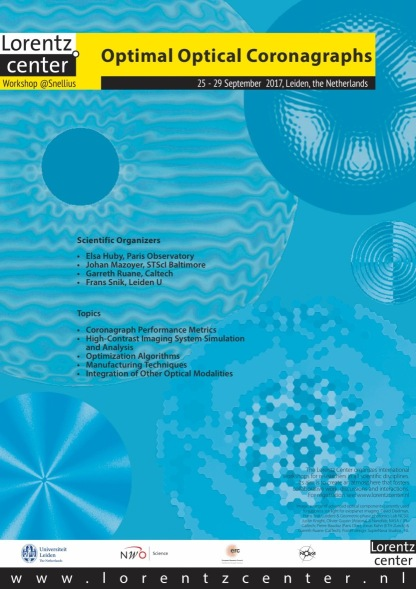
\includegraphics[width=1.\textwidth]{figures_CV/ooc_poster2_sm.jpg}
%  \end{mybox}
% \end{wrapfigure}
% \vspace{-0.2cm}
\begin{itemize} \itemsep 5pt
    \item[$\bullet$]\small Séminaire \textbf{``Haute Résolution Angulaire pour l'Astrophysique" (HRAA)} au LESIA (2020-)
    \item[$\bullet$] \small Organisateur et SOC : \textbf{National Capital Area Disks} (Baltimore, MD, Oct. 2018). \href{https://sites.google.com/view/ncad7-at-jhu/ncad7}{\underline{\textbf{Site internet}}}
    \item[$\bullet$] \small Organisateur et SOC : \textbf{Optimal Optical Coronagraphs (Leiden, NL, Sep. 2017)}. \href{https://www.lorentzcenter.nl/lc/web/2017/924/info.php3?wsid=924&venue=Snellius}{\underline{\textbf{Site internet}}}
    \item[$\bullet$]\small Séminaire \textbf{``Exoplanet Star and Planet Formation" (ESPF)} au STScI (2016-2018)
    \item[$\bullet$] \small SOC : \textbf{High Contrast Imaging from Space (Baltimore, MD, US, Nov 2016)}.  \href{http://www.cvent.com/events/high-contrast-imaging-in-space-workshop/event-summary-eb3bb6bd54a342c5a15678daa49be683.aspx}{\underline{\textbf{Site internet}}}
    \item[$\bullet$] \small Organisateur : \textbf{La très haute dynamique (Paris, Fr, Oct. 2012)}
\end{itemize}
\vspace{0.4cm}
%\textbf{Développement d'un logiciel pour la communauté}\\
%\vspace{-0.7cm}
%\begin{itemize} \itemsep -3pt % reduce space between items
%    \item \small Développement d'un \textit{pipeline} pour le consortium GPI pour traiter les disques avec l'instrument coronographique GEMINI/GPI. Ce code, dit de \textit{forward-modelling} permettra à terme d'identifier les effets sur la forme et la photométrie dus au traitement d'image.
%\end{itemize}


\textbf{Autres investissements}\\
\vspace{-0.1cm}
\begin{itemize} \itemsep 5pt
    \item[$\bullet$] \small Responsable de l'équipe haut-contraste du LESIA \hfill 2023 - 
    \item[$\bullet$] \small Comité d'experts du thème transverse exoplanètes de l'INSU \textbf{(CET exoplanètes)} \hfill 2023 - 
    \item[$\bullet$] \small \textbf{Roman:} Représentant adjoint du CNES au Community Participation Program (CPP) Team \hfill 2023 - 
    \item[$\bullet$] \small \textbf{SPHERE+:} Responsable du groupe de travail Focal Plane Wavefront Sensor \hfill 2022 - 
    \item[$\bullet$] \small Comité Scientifique de l'action Spécifique Haute résolution Angulaire de l'INSU \textbf{(ASHRA)} \hfill 2021 - 
    \item[$\bullet$] \small \textbf{Habitable Exoplanet Observatory (HabEx)}: Contributeur scientifique \hfill 2019
    \item[$\bullet$] \small \textbf{Large UV Optical Infrared Surveyor (LUVOIR)}: Contributeur scientifique \hfill 2019
    \item[$\bullet$] \small Participation au {\bf Telescope Allocation Committee} d'Hubble \hfill 2016
    % \item[$\bullet$] \small Membre du Study Analysis Groups (SAGs) \#19 de l'\textbf{Exoplanet Exploration Program Analysis Group} (ExoPAG). Le SAG numéro 19 regroupe des chercheurs pour définir de nouvelles métriques d'évaluation et de comparaison des méthodes de détection d'exoplanètes (Jensen Clem et al. 2017).
    % \item[$\bullet$] \small Organisation du \textbf{séminaire ``Exoplanet, Star and Planet Formation"} au STScI (2016 - 2018). Ce séminaire invite des chercheurs d'autres organismes chaque semaine au STScI.
    % \item[$\bullet$] \small Développement du \textbf{site internet du banc optique THD} de Meudon en Août 2014, dans l'objectif de faire connaître ses caractéristiques à l'international pour créer de nouvelles collaborations.
    \item[$\bullet$] \small Membre de l'IAU \hfill 2019 - 
    \item[$\bullet$] \small \textbf{Peer-review} pour le \textit{AJ}, \textit{A\&A}, \textit{MNRAS}, \textit{PASP} et \textit{Journal of Astronomical Telescopes, Instruments, and Systems}.
\end{itemize}

% \vspace{-0.35cm}
% \textcolor{RoyalBlue}{\section{\large REFERENCES}
% \vspace{-0.3cm}\hrule}
% \vspace{0.3cm}

% \vspace{0.5cm}
% \hspace{0.5cm}\parbox{0.08\linewidth}{\textbf{1.}}
% \parbox{0.46\linewidth}{\textbf{G\' erard Rousset}\\
% \textit{Professeur à l'université Paris Diderot} \\
% Directeur de ma thèse\\
% LESIA -- Observatoire de Paris, France\\
% gerard.rousset@obspm.fr}
% \parbox{0.42\linewidth}{\textbf{Anthony Boccaletti} \\
% \textit{Chargé de recherche CNRS}\\
% Proche collaborateur au LESIA\\
% LESIA -- Observatoire de Paris, France\\
% anthony.boccaletti@obspm.fr}


% \vspace{0.8cm}
% \hspace{0.5cm}\parbox{0.08\linewidth}{\textbf{2.}}
% \parbox{0.56\linewidth}{\textbf{Laurent Pueyo}\\
% \textit{Astronomer}\\
% Encadrant de mon premier post-doc\\
% Space Telescope Science Institute, Baltimore, MD, US\\
% pueyo@stsci.edu}


% \vspace{0.8cm}
% \hspace{0.5cm}\parbox{0.08\linewidth}{\textbf{3.}}
% \parbox{0.80\linewidth}{\textbf{John Trauger}\\
% \textit{Senior Research Scientist}\\
% PI de HST/WFPC2, scientifique en charge de WFIRST/CGI à JPL\\
% Jet Propulsion Laboratory, Pasadena, CA, US\\
% john.trauger@jpl.nasa.gov}

%%%%%%%%%%%%%%%%%%%%%%%%%%%%%%%%%%%%%%%%%%%%%%%%%%%%%%%%%%%%%%%%%%%%%%%%%%%%%%%%%%%%%%%%%%%%%%%%%%%%%%%%%%%%%%%%%%%%%%%%
%%%%%% SECTION MISC.
%%%%%%%%%%%%%%%%%%%%%%%%%%%%%%%%%%%%%%%%%%%%%%%%%%%%%%%%%%%%%%%%%%%%%%%%%%%%%%%%%%%%%%%%%%%%%%%%%%%%%%%%%%%%%%%%%%%%%%%%

%\vspace{-0.8cm}
%\textcolor{RoyalBlue}{\section{\large  SPORTS}
%\vspace{-0.35cm}\hrule}
%\vspace{0.35cm}
%\begin{itemize}\itemsep -3pt
%\item \textbf{Escrime} (15 ans de pratique en club)
%\item \textbf{Course à pied} (trails, semi-marathons, marathon)\\
%\end{itemize}

% %%%%%%%%%%%%%%%%%%%%%%%%%%%%%%%%%%%%%%%%%%%%%%%%%%%%%%%%%%%%%%%%%%%%%%%%%%%%%%%%%%%%%%%%%%%%%%%%%%%%%%%%%
% %
% %%%%% presentations
% %
% %%%%%%%%%%%%%%%%%%%%%%%%%%%%%%%%%%%%%%%%%%%%%%%%%%%%%%%%%%%%%%%%%%%%%%%%%%%%%%%%%%%%%%%%%%%%%%%%%%%%%%%%%
% \newpage
% \textcolor{White}{.}
% %\lhead{\textcolor{Gray}{J. MAZOYER}}
% \vspace{-1.5cm}
% \begin{center}
% \begin{LARGE}
% \textbf{Liste des présentations}\\
% \end{LARGE}
% \end{center}
% \setcounter{section}{0}

% \vspace{-0.8cm}
% \textcolor{RoyalBlue}{\section{PRÉSENTATIONS INVITÉES}
% \vspace{-0.25cm}\hrule}
% \vspace{0.6cm}


% \begin{etaremune}
% \item ``Active correction of aperture discontinuities and observation of circumstellar debris disks with GPI", IPAC seminar, Pasadena, FR \textbf{Avr. 2019}

% \item ``High contrast imaging: from active correction to observation of circumstellar debris disks", LESIA seminar, Meudon, FR \textbf{Mar. 2019}

% \item ``Wavefront control and sensing for the direct imaging of exoplanets", JPL seminar, Pasadena, FR \textbf{Dec. 2018}

% \item ``High contrast imaging: from active correction to observation of circumstellar debris disks", IPAG, Grenoble, FR \textbf{Mar. 2018}

% \item ``High contrast imaging: active correction of aperture discontinuities", Carnegie DTM Astronomy Seminar, Washington, DC, USA \textbf{Fev. 2018}

% \item ``High contrast imaging: active correction of aperture discontinuities", STScI/JHU CoolSci Talk Series, Baltimore, MD, USA \textbf{Fev. 2017}

% \item ``High contrast imaging: from active correction to observation of circumstellar debris disks", IRAP seminar, Toulouse FR \textbf{Mar. 2017}

% \item ``Correction of aperture discontinuities for the direct imaging of exoplanets and circumstellar disks", CRAL séminar, Lyon, FR \textbf{Sep. 2016}

% \item ``Active Correction of Aperture Discontinuities (ACAD) for Space Telescope Pupils: A parametrical analysis", Vortex coronagraph workshop 2, Caltech, Pasadena, CA, US \textbf{Juil. 2016}
% \end{etaremune}

% \vspace{-0.8cm}
% \textcolor{RoyalBlue}{\section{CONFÉRENCES ET ATELIERS INTERNATIONAUX}
% \vspace{-0.25cm}\hrule}
% \vspace{0.6cm}


% \begin{etaremune}

% \item ``The surprising scattering phase function of the HR 4796 debris disk ", American Astronomical Society 233 conference, Seattle, CA, US \textbf{Jan. 2019}

% \item ``Current Limitations and Perspectives for Direct Imaging Instrumentation for Future Space-Based Telescopes", Sagan/Michelson Fellows Symposium, Pasadena, CA, US \textbf{Nov. 2018}

% \item ``High-Contrast Imaging of the HR 4796 Debris Disk with the Gemini Planet Imager", NCAD 7 conference, Baltimore, MD, US \textbf{Sep. 2018}

% \item ``Forward modeling techniques for spectra retrieval of circumstellar debris disks", American Astronomical Society 231 conference, Washington, DC, US \textbf{Jan. 2018}

% \item ``Beam shaping coronagraphs", OOC workshop, Leiden, NL \textbf{Sep. 2017}

% \item ``The HiCAT testbed", OOC workshop, Leiden, NL \textbf{Sep. 2017}

% \item ``Capabilities of ACAD-OSM, an active method for the correction of aperture discontinuities", SPIE Conference, San Diego, CA, US \textbf{Août 2017}

% \item ``Fundamental limits to high-contrast wavefront control", SPIE Conference, San Diego, CA, US \textbf{Août 2017}

% \item ``A new active method to correct for the effects of complex apertures on coronagraph performance", American Astronomical Society 229 conference, Grapewine, TX \textbf{Jan. 2017}

% \item ``Correcting for aperture discontinuities with deformable mirrors for futur space telescopes", High Contrast Imaging in Space workshop, STScI, Baltimore, MD \textbf{Nov. 2016}

% \item ``Deep inside circumstellar disks investigating the NICI archive", NCAD 6 conference, Carnegie DTM, Washington DC, US \textbf{Juil. 2016}

% \item ``Active correction of aperture discontinuities (ACAD) for space telescope pupils: a parametric analysis". SPIE Conference, Techniques and Instrumentation for Detection of Exoplanets VII. San Diego, CA, US. \textbf{Août 2015}.

% \item ``THD bench : description and latest results". Coronagraphs and Wavefront Control Workshop. Leiden, Netherlands, \textbf{Oct. 2014}.

% \item ``Direct detection of exoplanets in polychromatic light with a Self-coherent camera". SPIE Conference, Techniques and Instrumentation for Detection of Exoplanets VI. San Diego, CA, US. \textbf{Août 2013}.

% \item ``Deformable mirror analysis for direct imagery of exoplanets". Journées recherche et industrie de l’optique adaptative 6. Villetaneuse, France. \textbf{Juil. 2013}.

% \item ``Self-Coherent Camera : principe", Workshop ``Très haute Dynamique". Meudon, France. \textbf{Sept. 2012}.

% \item ``La Self-Coherent Camera : estimation de front d'onde en plan focal pour la détection d'exoplanètes en imagerie directe". Journées recherche et industrie de l'optique adaptative 5. Marseille, France. \textbf{Juil. 2012}.
% \end{etaremune}

% \vspace{-0.8cm}
% \textcolor{RoyalBlue}{\section{SÉMINAIRES}
% \vspace{-0.25cm}\hrule}
% \vspace{0.6cm}

% \begin{etaremune}
% \item NASA's Goddard Space Flight Center seminar, MD, US. ``A new active method to correct for the effects of complex apertures on coronagraph performance" \textbf{Jan. 2017}

% \item ESO TMT seminar, Santiago, CL. ``A new active method to correct for the effects of complex apertures on coronagraph performance" \textbf{Nov. 2016}

% \item Séminaire de l'OCA, Nice, FR. ``Correction of aperture discontinuities for the direct imaging of exoplanets and circumstellar disks" \textbf{Août 2016}

% \item Space Telescope Science Institute post-doc Jamboree, MD, US. ``Deep inside circumstellar disks: high-contrast instrumental techniques and archival data analysis" \textbf{Fév. 2016}.

% \item Wine \& Cheese seminar, Johns Hopkins University, MD, US. ``Deep inside circumstellar disks: high-contrast instrumental techniques and archival data analysis" \textbf{Avr. 2015}.

% \item LOOM Seminar, LAM, Marseille, France. ``Deep inside circumstellar disks: high contrast instrumental techniques and data analysis using NICI". \textbf{Mars 2015}.

% \item STScI science coffee seminar, Baltimore, MD, US. ``Deep inside circumstellar disks with the GEMINI/NICI coronagraphic instrument"  \textbf{Jan. 2015}.

% \item Astrium optical group seminar, Toulouse, France. ``Self Coherent Camera and THD bench"  \textbf{Oct. 2013}.

% \item Séminaire Haute Résolution angulaire, LESIA, Obs. de Paris, France. ``The self-coherent camera: speckle nulling in polychromatic light for the direct detection of exoplanets" \textbf{Oct. 2013}.

% \item CNES optical group seminar, ``Self Coherent Camera and THD bench", Toulouse, France \textbf{Oct. 2013}.

% \item Journées des jeunes chercheurs du CNES (JC2), Toulouse, France. ``La Self-Coherent Camera : imagerie directe par coronographie pour la détection et l'analyse spectrale d'exoplanètes",  \\
% \textbf{Récompensée par le prix de la meilleure présentation} \textbf{Oct. 2013}.

% \item Journées des thèses du LESIA, Obs de Paris, France. Deux présentations, en \textbf{Mars 2012} et \textbf{Avr. 2013}.

% \item Conférence ``Elbereth" des doctorants en astronomie et astrophysique d'Île-de-France, IAP, Paris, France. Trois présentations en \textbf{Déc. 2011, 2012 et 2013}.\\

% \end{etaremune}


% \textcolor{RoyalBlue}{\Large{\bf + 9 posters en conférences internationales}}


% \vspace{-0.8cm}
% \textcolor{RoyalBlue}{\section{PRÉSENTATIONS GRAND PUBLIC}
% \vspace{-0.25cm}\hrule}
% \vspace{0.6cm}

% \begin{enumerate}\itemsep 3pt
% \item[$\bullet$]  ``Extremely Large Telescopes : des cathédrales pour l'astronomie". CERN, Genève, Suisse \textbf{Août 2014}.

% \item[$\bullet$] ``Des œufs dans l'espace". Palais de la découverte, Paris, France \textbf{Mai 2016}.

% \item[$\bullet$] ``Excréments dans l'espace". Palais de la découverte, Paris, France \textbf{Mai 2017}.
% \end{enumerate}

% %\begin{enumerate}
% %
% %\item ``Correcting for the effects of pupil discontinuities with the ACAD method", SPIE Conference, Edinburgh, UK \textbf{Juin 2016}
% %
% %\item ``Detection and Characterization of Exoplanets using Projections on Karhunen-Loeve Eigenimages: Forward Modeling", AAS conference, Kissimmee, FL, US. \textbf{Jan. 2016}.
% %
% %\item ``Propagation Simulations for Two-Mirror Wavefront Correction and Active Compensation of Aperture Discontinuities", In the spirit of Lyot Conference, Montreal, Canada. \textbf{Juil. 2015}.
% %
% %\item ``Deep Inside Circumstellar Disks Investigating the Near-Infrared Coronagraphic Imager Archive", In the spirit of Lyot Conference, Montreal, Canada. \textbf{Juil. 2015}.
% %
% %\item ``Is the HD~15115 disk really asymmetrical ?", Thirty years of beta Pic and debris disks studies conference. Paris, France. \textbf{Sept. 2014}.
% %
% %\item ``Deformable mirror interferometric analysis for the direct imagery of exoplanets". SPIE Conference, Adaptive Optics Systems IV, Montreal, Canada. \textbf{Juil. 2014}.
% %
% %\item ``Direct detection of exoplanets in polychromatic light with a Self-coherent camera". Third AO4ELT Conference, Firenze, Italy. \textbf{Mai 2013}.
% %
% %\item ``Experimental parametric study of the self-coherent camera". SPIE Conference, Space Telescopes and Instrumentation 2012: Optical, Infrared, and Millimeter Wave. Amsterdam, Netherlands. \textbf{Juil. 2012}.
% %
% %\end{enumerate}

\end{document}